En 2017, une cryptomonnaie adossée à la \textit{\gls{blockchain}} Solana a émergée avec des caractéristiques
similaires à \gls{Ethereum} : \textit{\gls{blockchain}} publique, \textit{\gls{smart contract}s}.\\
Solana est devenue de facto une \textit{\gls{blockchain}} concurrente à \gls{Ethereum} et est aujourd'hui 
la onzième \textit{\gls{blockchain}} en terme de capitalisation selon l'aggrégateur de marché Coinmarketcap.\\
Un besoin d'échanger des \gls{actif}s entre les \textit{\gls{blockchain}s} \gls{Ethereum} et Solana est apparu, 
d'où l'introduction en 2020 de la première version de \gls{Wormhole}.
Initialement, \gls{Wormhole} v1 a été concu comme un \textit{bridge} entre \gls{Ethereum} et Solana.
Depuis, \gls{Wormhole} s'est développé au-delà de Solana avec le lancement d'une deuxième version en 2021 
en tant que protocole générique de passage de messages.\\
À l'écriture de ce rapport, 22 \cite{wormholeNetwork} \textit{\gls{blockchain}s} sont compatibles avec \gls{Wormhole} 
dont : BNBChain, \gls{Ethereum}, Moonbeam, Polygon, Solana...\\
Le protocole émet un message à partir d'une \textit{\gls{blockchain}} source qui est validé par un réseau de 
gardiens.\\ 
Le message est ensuite envoyé à la \textit{\gls{blockchain}} cible pour être traité.

\subsubsection{VAA (\textit{Verified action approval})}

Lorsqu'un \textit{\gls{smart contract}} envoie un message \textit{crosschain} comme un verrouillage
de jetons sur une \textit{\gls{blockchain}} source et une demande de frappe de jetons sur une 
\textit{\gls{blockchain}} cible, celui-ci interargit avec un \textit{core contract} \cite{wormholeCoreContract}.
Un \textit{core contract} est déployé sur toutes les \textit{\gls{blockchain}s} compatibles avec le protocole 
\gls{Wormhole}. Tout \textit{core contract} est observé par le réseau de gardiens.
Un message \gls{Wormhole} est émis grâce à la fonction \textit{publishMessage()} prenant en entrée le \textit{payload}.
La sortie de cette fonction est un \textit{sequence number}, un numéro d'index unique pour le message.
Combiné à l'adresse du contrat de l'émetteur et à l'identifiant de la chaîne de l'émetteur, le message 
correspondant peut être récupéré auprès d'un nœud du réseau de gardiens.\\
Un message \gls{Wormhole} est vérifié grâce à la fonction \textit{parseAndVerifyVAA()} prenant en entrée le message.
Selon la validité de l'entrée, la fonction retourne en sortie le \textit{payload} ou une exception.

\acrshort{vaa} \cite{wormholeVAA} est la primitive de messagerie de base de \gls{Wormhole}. Un VAA contient une en-tête 
ainsi qu'un \textit{body}. L'en-tête contient l'index des gardiens ayant signés le message et la collection des signatures.
L'en-tête permet au \textit{core contract} de vérifier l'authenticité du VAA.
Quant au \textit{body}, il contient des informations comme le numéro d'identification de la chaîne 
\gls{Wormhole} du contrat émetteur, l'adresse du contrat émetteur, le \textit{sequence number} 
et le \textit{payload}.\\ 5 \textit{payloads} peuvent être utilisés dont \textit{Transfer} et 
\textit{AssetMeta}, attestant les méta-données du jeton.\\
Le \textit{payload AssetMeta} est obligatoire avant un premier transfert.
En effet, le \textit{payload Transfer} n'informe pas la chaîne B des meta-données du jeton verrouillé.
En l'absence de connaissance de ces informations, il n'est pas possible pour la \textit{\gls{blockchain}} B 
de frapper la quantité correcte de jetons.\\
Si l'on souhaite ensuite transférer des jetons depuis une \textit{\gls{blockchain}} A vers une 
\textit{\gls{blockchain}} B, il faut verrouiller les jetons sur A et les frapper sur B.
D'où l'utilisation du \textit{payload Transfer} contenant des informations comme la 
quantité de jetons transférés, l'adresse de la chaîne d'origine et de destination, 
le numéro d'identification de la chaîne d'origine et de destination..
Une preuve doit être fournie que les jetons sur A sont verrouillés avant que la frappe puisse 
avoir lieu sur B. La signature des gardiens sur le VAA correspondant est la preuve apportée à 
la \textit{\gls{blockchain}} B que le verrouillage a bien été effectué et que la frappe de jetons sur 
B est légitime.

\subsubsection{Gardiens}

Un gardien \cite{wormholeGuardian} est une autorité de confiance qui a comme rôle de valider 
(par une signature) le \textit{payload} contenu dans un VAA.
Comme évoqué précédemment, le réseau de gardiens observe tous les messages \textit{crosschain} via la 
surveillance des \textit{core contracts}.
Le réseau de gardiens est composé de 19 gardiens à parts égales sans chef (\textit{leaderless}).
Il est conçu pour servir d'oracle à \gls{Wormhole} et est l'élement le plus critique de l'écosystème.
Si une majorité de deux tiers ou plus des gardiens signent le même VAA, alors le consensus est atteint : 
le VAA est automatiquement considéré valide par  tous les contrats \gls{Wormhole} sur toutes les 
\textit{\gls{blockchain}s} et le \textit{payload} est actionné. 
Chaque gardien utilise un algorithme de signature à courbe elliptique : ECSDA pour 
\textit{Elliptic Curve Signature Digital Algorithm}.
Plus précisément, chaque gardien se réfère à «secp256k1» comme paramètres de la courbe elliptique, 
aussi utilisé par les \textit{\gls{blockchain}s} \gls{Bitcoin} et \gls{Ethereum}.\\
Le modèle de consensus utilisé est une \textit{Proof of Authority} (PoA) avec un système de 
\textit{multisignature} M/N \cite{wormholeChainswap}, c'est à dire que M clefs parmi N sont nécessaires 
pour signer un VAA. Ce modèle permet un traitement rapide des transactions et une dispense de participation monétaire, par rapport à la preuve de travail (PoW) et la preuve 
de participation (PoS). Cependant, il présente également des désavantages : le système est par 
\textit{design} centralisé et dépend d'un petit groupe de nœuds pouvant créer un point de 
défaillance unique par l'utilisation commune d'une fonction vulnérable. Il est questionnable de restaurer des tiers de confiance dans le cadre d'un système 
devenu populaire grâce à l'absence de tels autorités. \gls{Wormhole} justifie la décentralisation de leur 
système \cite{wormholeGuardian} par la présence de plusieurs parties (et non d'un seul) dans le contrôle du réseau.
Selon notre analyse, la décentralisation résulte de l'absence d'un ou plusieurs tier(s) de confiance lorsque deux parties 
souhaitent réaliser une transaction.

\subsubsection{Relais}

Un relai \cite{wormholeRelayer} est un processus qui délivre un VAA vers une destination.
Les relais ne sont ni de confiance, ni privilégiés, ils écoutent directement le réseau de gardiens 
via l'intermédiaire d'un processus espion. Ces relais ne peuvent pas compromettre l'intégrité d'un VAA 
car une altération serait détectée lors du processus de vérification des signatures. Cependant, il n'est 
pas assuré qu'un relai transmette un VAA à destination, d'où une perte de disponibilité. Il est conseillé
d'héberger soi-même ces relais pour supporter son application.

\begin{figure}[h!]
    \centering
    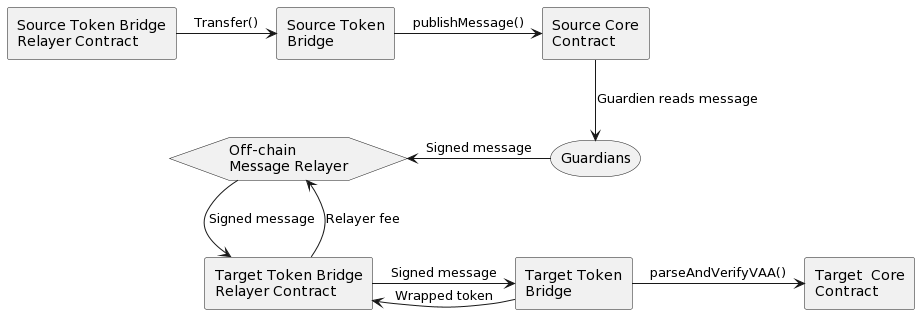
\includegraphics[scale=0.5]{centralisation/uml_design_v2.png}
    \label{fig:wormholeDesign}
    \caption{Architecture \gls{Wormhole} \cite{wormholeArch}}
  \end{figure}

% @startuml
% rectangle r1 as "Source Token Bridge 
% Relayer Contract"
% rectangle r2 as "Source Token 
% Bridge"
% rectangle r3 as "Source Core 
% Contract"
% storage "Guardians" as r4
% hexagon r5 as "Off-chain 
% Message Relayer" 
% rectangle r6 as "Target Token Bridge 
% Relayer Contract"
% rectangle r7 as "Target Token 
% Bridge"
% rectangle r8 as "Target  Core 
% Contract"

% r1 -> r2 : Transfer()
% r2 -> r3 : publishMessage()
% r3 -do-> r4 : Guardien reads message
% r4 -left-> r5 : Signed message

% r5 -do-> r6 : Signed message
% r6 -> r5 : Relayer fee

% r6 -> r7 : Signed message
% r7 -> r6 : Wrapped token

% r7 -> r8 : parseAndVerifyVAA()
% @enduml


